\chapter{Systemarchitektur}
\section{Klassendiagramm des Projekts}

In diesem Abschnitt wird das Klassendiagramm der Ampelschaltung (siehe Abbildung \ref{fig:grafik8}) erläutert. Es wird darauf eingegangen, wie die einzelnen Klassen in Beziehung zueinanderstehen und wie diese gruppiert werden können.\\
\\
Das Klassendiagramm lässt sich in vier Bereiche unterteilen:\\

\begin{itemize}
	\item Auswahl Betriebsmodus (blau)
	\item Steuerung Farben (grün)
	\item Output (rot)
	\item Input (schwarz)\\
\end{itemize}

Der Bereich \glqq Auswahl Betriebsmodus\grqq{} bildet die Logik der beiden Betriebsmodi ab, in denen sich die Ampel befinden kann. Zum einen der aktive Modus, in welchem die Ampel die Farben durchschaltet und zum anderen den Modus, in welchem die Ampel orange blinkt. Der Bereich \glqq Steuerung Farben \grqq{} übernimmt die Aufgabe die Zustände im Hinblick auf die Farben der Ampel bereitzustellen. Die Ampel kann Rot ausgeben, Rot-Organge, Orange, Grün oder ausgeschaltet sein. Der Output übernimmt die Funktion, die einzelnen Farben zu setzen und dies entweder software- oder hardwaremäßig. Der Input übernimmt die Aufgabe die Benutzereingabe bereitzustellen, die ebenso entweder software- oder hardwaremäßig eingegeben werden kann. Die Klasse GPIO, die nicht in einen der Bereiche zugeordnet wird, bildet die Schnittstelle für den Hardwarezugriff ab.\\
\\
Hierarchisch ganz oben ist die Kontextklasse \glqq Traffic Light\grqq{} zu sehen. Ein Objekt dieser Klasse wird in der\: \texttt{main()} erstellt und beinhaltet die Logik der gesamten Ampelschaltung. Wird die\: \texttt{Handle()} Funktion dieses Objekts aufgerufen, läuft die Ampelschaltung wie gefordert ab. Die Aufgabe Benutzereingaben einzulesen wird an das Interface \glqq InputFormat\grqq{} delegiert. Je nachdem, ob eine Hardware angeschlossen ist, liefern die Klassen \glqq SoftwareInput\grqq{} und \glqq HardwareInput\grqq{} den jeweiligen Tasterwert, bzw. die Tastatureingabe. Die Klasse \glqq UserButtons\grqq{} frägt beide Pins (für die beiden Taster) ab und stellt der Klasse \glqq HardwareInput\grqq{} nur einen Wert zur Verfügung, der die beiden Tasterzustände abbildet. Damit die Klasse \glqq UserButtons\grqq{} auf die Registerinhalte des Mikrocomputers zugreifen kann, steht sie in Beziehung mit der Klasse \glqq GPIO\grqq{}. Ein Objekt der \glqq Traffic Light\grqq{} Klasse kann den Zustand in Betrieb oder außer Betrieb annehmen. Über das Interface \glqq state\grqq{} werden die Zustandsklassen \glqq flashing\grqq{} und \glqq active\grqq{} hierfür bereitgestellt. Diese beiden Klassen greifen über das Interface \glqq LightControl\grqq{} auf die Farbenklassen \glqq Off\grqq{}, \glqq Red\grqq{}, \glqq RedAmber\grqq{}, \glqq Amber\grqq{} und \glqq Green\grqq{} zu. Diese Unterklassen sind dafür verantwortlich, dass die Ampel den Farbzustand annimmt. Des Weiteren bieten diese Klassen die Funktion an, Objekte für den nächsten Farbzustand zurückzuliefern. Noch eine Hierarchieebene weiter darunter greifen die Farbklassen über das Interface \glqq OutputFormat\grqq{} auf die \glqq SoftwareOutput\grqq{} bzw. auf die Klasse \glqq HardwareOutput\grqq{} zu. Diese realisieren die Ausgabe der Ampelschaltung. Im Fall, dass Hardware angeschlossen ist, greift die \glqq HardwareOutput\grqq{} Klasse über die \glqq UserLEDs\grqq{} Klasse auf die \glqq GPIO\grqq{} Klasse zu. Damit werden die entsprechenden Bits in den Registern des Mikrocontrollers gesetzt, damit die entsprechenden Pins der LEDs auf HIGH geschaltet werden können.

\begin{figure}[H] 
	\centering
	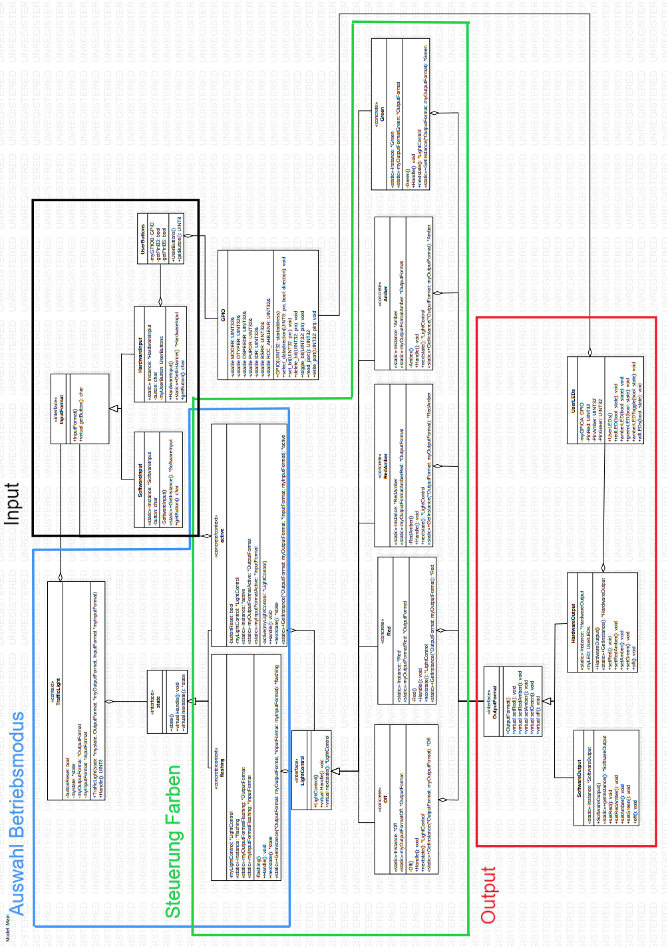
\includegraphics[width=0.95\textwidth]{images/08.png}
	\caption{Klassendiagramm der Ampelsteuerung \protect \\ Quelle: Eigene Darstellung }
	\label{fig:grafik8}
\end{figure}

\section{Zustandsautomat}

\begin{figure}[H] 
	\centering
	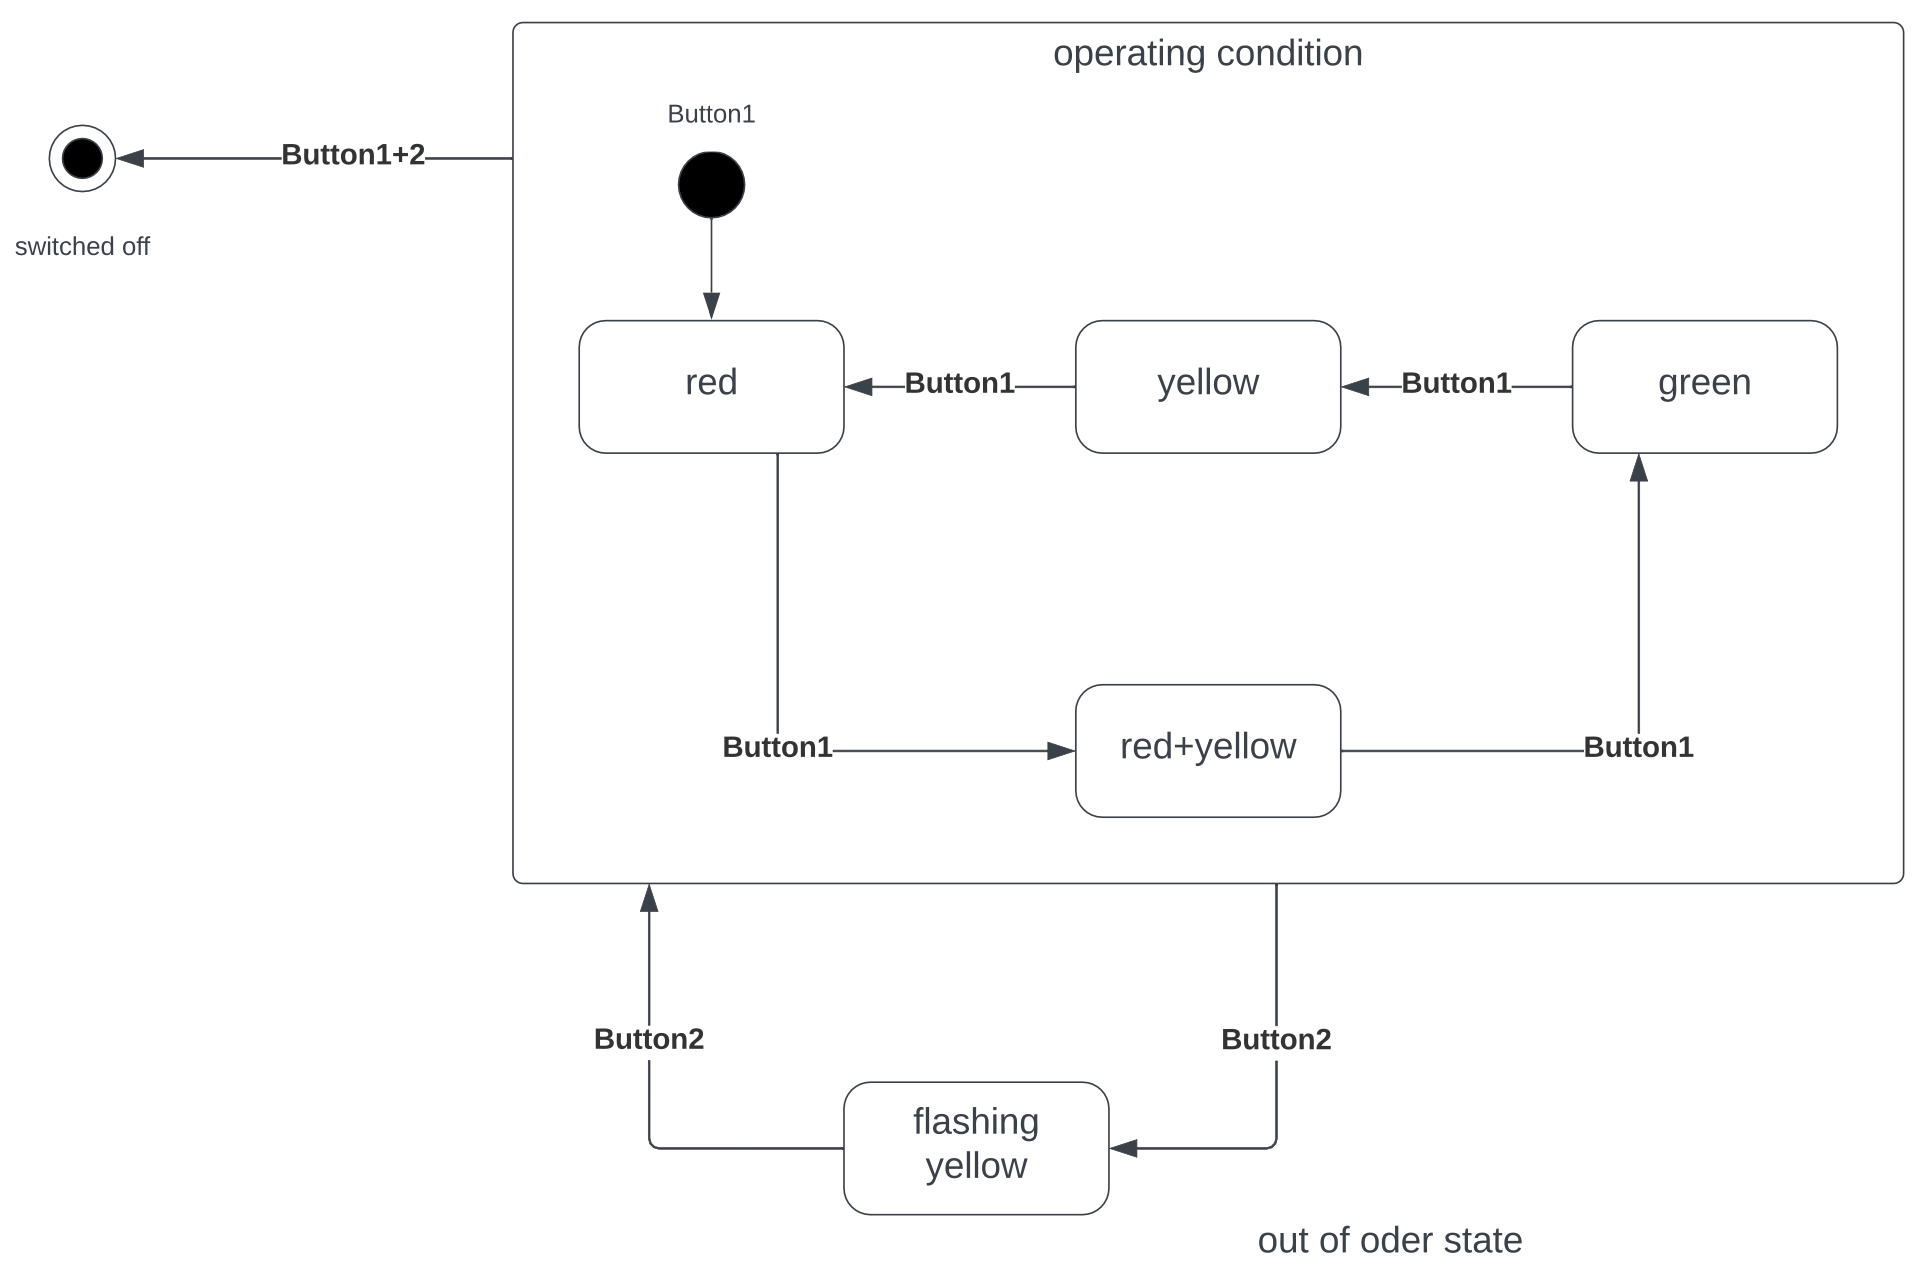
\includegraphics[width=1.0\textwidth]{images/03.png}
	\caption{Zustandsautomat der Ampelsteuerung \protect \\ Quelle: Eigene Darstellung }
	\label{fig:grafik3}
\end{figure}


Ein Zustandsdiagramm ist eines der 14 Diagrammarten der Sprache UML für Software und andere Systeme. Es ermöglicht dem Entwickler sich einen Gesamtüberblick über die Zustände und Operationen, welche in einem Projekt/Programm erfolgen sollen, zu verschaffen. \\
Die zu implementierende Ampelsteuerung soll zwei Zustände \glqq In Betrieb\grqq{} und \glqq Außer Betrieb\grqq{} annehmen können. Im Betrieb soll die Ampelsteuerung die Ampelphasen Rot, Rot-Gelb, Grün und Gelb durchlaufen (siehe \autoref{fig:grafik3}). Die Ampelphasen sollen per Taster \glqq T1\grqq{} oder Tastatureingabe \glqq F\grqq{} gesteuert werden. Zwischen jeder Ampelphase kann die Ampelsteuerung mit dem Taster \glqq T2\grqq{} oder Tastatureingabe \glqq B\grqq{} in den \glqq Außer Betrieb\grqq{} Zustand gesetzt werden. Innerhalb dieses Zustandes, soll die gelbe LED blinken (siehe \autoref{fig:grafik3}). Immer wenn die Ampelsteuerung neugestartet oder in den Betriebsmodus \glqq In Betrieb\grqq{} wechselt, soll sie in der roten Ampelphase starten.
